\chapter{Samplers: Framework Android} \label{cap:samplers}

\section{Propuesta general}

\subsection{Descripción del problema}
En la descripción del Estado del Arte (Sección \ref{sec:estado_arte}), se describen algunas herramientas que sirven de soporte a los científicos para incluir ciencia ciudadana en sus proyectos, y facilitar la recolección de la información o la recolección de muestras a través de formularios web o de aplicaciones para dispositivos móviles. Estas herramientas de soporte existen porque la simplicidad de utilización de los dispositivos móviles es ideal para que los científicos ciudadanos participen en la recolección de muestras, pero el desarrollo de estas aplicaciones puede ser una limitante para algunos proyectos por su complejidad técnica. \cite{kim2013sensr}
Para evitar que el desarrollo de una aplicación móvil sea limitante a la hora de incluir ciencia ciudadana en proyectos de investigación, se propone un framework que permita la creación de una aplicación móvil de manera sencilla para la recolección de muestras realizada por científicos ciudadanos.
El objetivo principal es permitir crear una aplicación móvil de ciencia ciudadana sin tener conocimientos de programación. Por ejemplo, desde una página web armar el protocolo de recolección de las muestras y con el mismo poder generar una aplicación móvil que sirva para tomar las muestras siguiendo dicho protocolo.

El protocolo de recolección debe estar compuesto por los diferentes pasos necesarios para tomar la muestra con la aplicación. Estos pasos deben permitir:
\begin{itemize}
\item capturar una foto, un video o un audio.
\item tomar la posición del GPS o grabar un recorrido con el GPS.
\item contestar una pregunta con respecto a la muestra. Esta pregunta puede tener una o múltiples respuestas posibles.
\item introducir anotaciones (texto).
\item seleccionar una fecha o una hora.
\item mostrar información de orientación para la toma de la muestra.
\end{itemize}

Las muestras recolectadas con la aplicación deben ser enviadas por Internet a un servidor web previamente configurado para dicho propósito.

La aplicación generada debe ser una aplicación nativa, y no una solución web por ejemplo, para poder aprovechar mejor las características de los dispositivos móviles (cámara, GPS, etc.). Además se debe contemplar que al momento de tomar una muestra es posible que no se cuente con conexión a Internet, pero igualmente se debe permitir la toma de la muestra y se la debe almacenar en el dispositivo móvil hasta que haya conexión a Internet y pueda ser enviada al servidor web.

La aplicación generada servirá para tomar muestras siguiendo el protocolo de recolección especificado, almacenarlas y empaquetarlas en el dispositivo móvil hasta que puedan ser enviadas al servidor web.

Además se deberá contemplar algún mecanismo para poder mostrar ayuda para el usuario final de la aplicación (el científico ciudadano) que sirviera de orientación para tomar la muestra. 

También se debe contemplar algún mecanismo de identificación del usuario que toma las muestras, con usuario y contraseña, o con alguna red social (Facebook, Twitter, Instagram, Google, etc.) para así poder darle una devolución mostrándole información, o incentivarlo para que siga participando del proyecto a través de gamificación por ejemplo.



\subsection{Alcance de la solución propuesta}
En un principio, Samplers se pensó para que un científico pudiera crear su propia aplicación móvil de ciencia ciudadana sin tener conocimientos de programación. 
La idea inicial era que, mediante una aplicación web, el científico pudiera armar el protocolo de recolección de las muestras de manera visual e intuitiva, y se generara un archivo de configuración para el framework de este trabajo: Samplers. 
Con el archivo de configuración se pasaría a Samplers y se generaría la app para Android (el archivo APK para instalarla). 
Pero de esta forma el alcance de la tesis era muy grande, por lo que se decidió quitar la parte de la aplicación web y suponer que el archivo de configuración ya viene armado.

Como se mencionó antes se requerían aplicaciones nativas, pero abarcar los 3 sistemas operativos móviles más usados en ese momento (Android, iOS y Windows Phone) era mucho para el alcance de esta tesis, por lo que se decidió optar por Android, que era el sistema operativo móvil más usado en ese momento. Según una estadística elaborada por Gartner Inc., empresa consultora y de investigación de las tecnologías de la información, sobre las ventas de smartphones a nivel mundial en el último trimestre de 2016\cite{gartner}, mas del 80\% de las mismas fueron de celulares con Android, y ese porcentaje fue creciendo hasta obtener una cuota del mercado del 88\% a nivel mundial a mediados de 2018. En la actualidad, en Argentina esa cuota de mercado es mas grande, llegando al 93\% según datos publicados por Carrier y Asociados, estudio profesional dedicado a la información y el análisis de mercado para productos y servicios vinculados a internet, en su reporte Mercado Celular Argentino 2019\cite{carrier}.

Para desarrollar aplicaciones móviles para la plataforma Android, el entorno de desarrollo integrado (IDE por sus siglas en inglés) oficial es Android Studio\cite{androidStudio}, por lo que Samplers utiliza el mismo para la generación de la app. Android Studio ha sido publicado de forma gratuita bajo Licencia Apache 2.0 y está disponible para las plataformas Microsoft Windows, MacOS y GNU/Linux.

\subsection{Descripción de la solución propuesta: Samplers}
Samplers es un framework que permite construir, de manera sencilla, aplicaciones Android (apps) para recolectar muestras en proyectos de Ciencia Ciudadana. Brinda una solución simple al problema de la recolección de la muestra aprovechando las funcionalidades de los dispositivos móviles.

Configurando el Workflow (que representa el protocolo de recolección en Samplers) y unos parámetros más, con Samplers se puede generar una app lista para ejecutarse en un dispositivo móvil Android. Esta app generada sirve para tomar muestras siguiendo el Workflow especificado, y las almacena en el dispositivo móvil hasta que puedan ser enviadas a un servidor web previamente configurado.

La app generada contiene, entre otras cosas, una Activity principal que muestra un texto de bienvenida (configurable) y un botón para tomar una muestra. Al presionar dicho botón se llama a la Activity encargada de tomar las muestras siguiendo el Workflow configurado. Esta Activity va mostrando en pantalla un Fragment por cada «paso» dentro del Workflow (Steps en Samplers). Cada uno de estos Fragments va interactuando con el usuario final de la app, el científico ciudadano\footnote{Se diferencia al usuario de Samplers, que es el que desea generar una app para recolectar muestras en un proyecto de ciencia ciudadana, del usuario final de la app, que es quien va a usar la app generada, que sería el científico ciudadano.}, para completar cada uno de los Steps del Workflow y así tomar la muestra (Sample en Samplers).

Para configurar el Workflow y los demás parámetros que necesita Samplers para generar la app, se debe completar un archivo de configuración llamado SamplersConfig.json.

Por ejemplo, si se desea crear una aplicación para hacer un relevamiento de las zonas con presencia del mosquito transmisor del Dengue (Aedes Aegypti), solicitando a los científicos ciudadanos que tomen fotos de los mosquitos que encuentren con las características del mosquito Aedes Aegypti, junto con la posición del GPS del dispositivo móvil. De esta manera se podría identificar al mosquito con la foto, y con la posición GPS armar un mapa de los avistajes. Para recolectar estas muestras se podría definir el protocolo de recolección de la siguiente manera:

\begin{enumerate}

\item Mostrar al científico ciudadano las características del mosquito Aedes Aegypti para que las pueda comparar con el mosquito encontrado (para evitar el envío de fotos innecesarias).

\item Pedir al científico ciudadano que tome una foto desde arriba del mosquito.

\item Pedir al científico ciudadano que tome una foto del costado del mosquito.

\item Pedir al científico ciudadano que tome la posición del GPS

\end{enumerate}

Para representar este protocolo de recolección se debería configurar el Workflow en el archivo de configuración para Samplers de la siguiente manera: 

\begin{figure}[H]
  \centering
    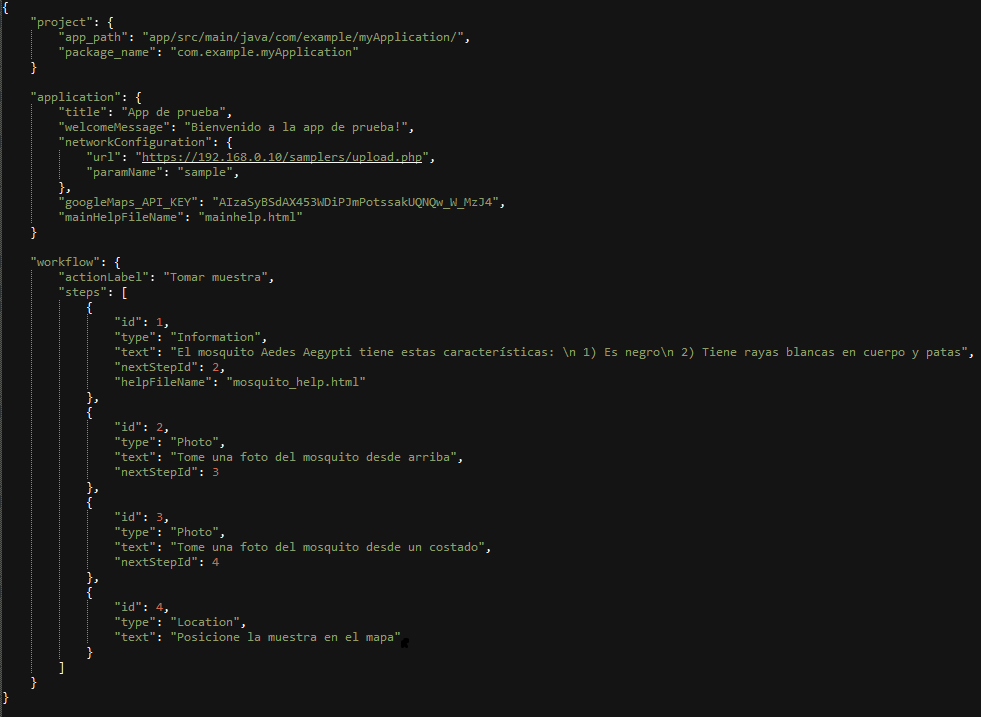
\includegraphics[width=\textwidth]{05-implementacion/archivo_config_app_ejemplo.png} 
   \caption{Archivo de configuración para Samplers de la app ejemplo}
\end{figure}


Con este archivo de configuración, Samplers generará el código necesario para la app, que al compilarla y ejecutarla en un dispositivo móvil Android se verá como muestra la siguiente imagen:



\begin{figure}[H]
	\begin{center}
   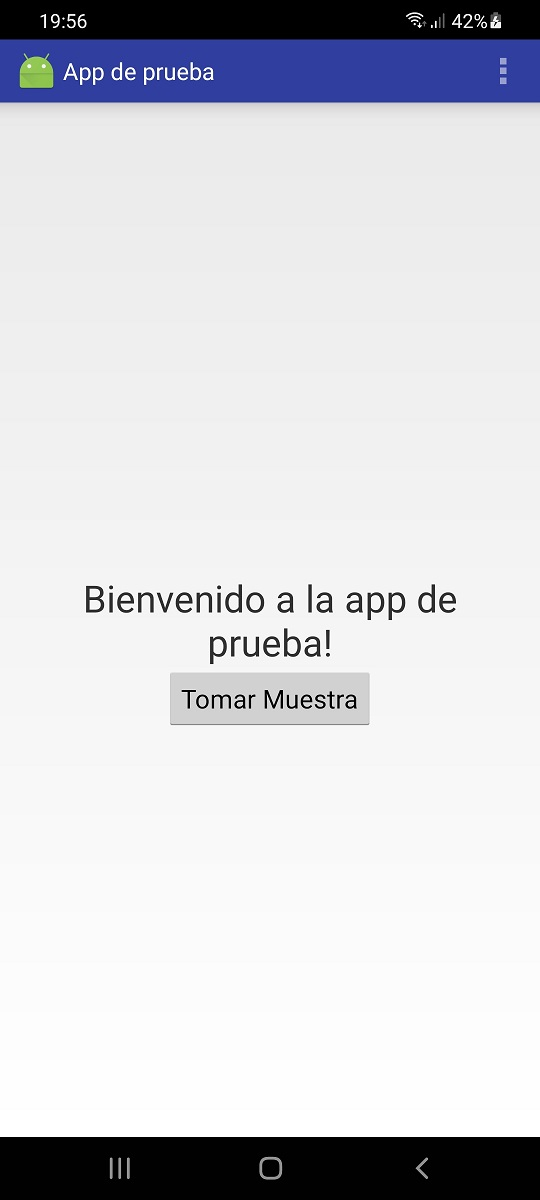
\includegraphics[scale=0.3]{05-implementacion/app_generada_ejemplo1.jpg} 
   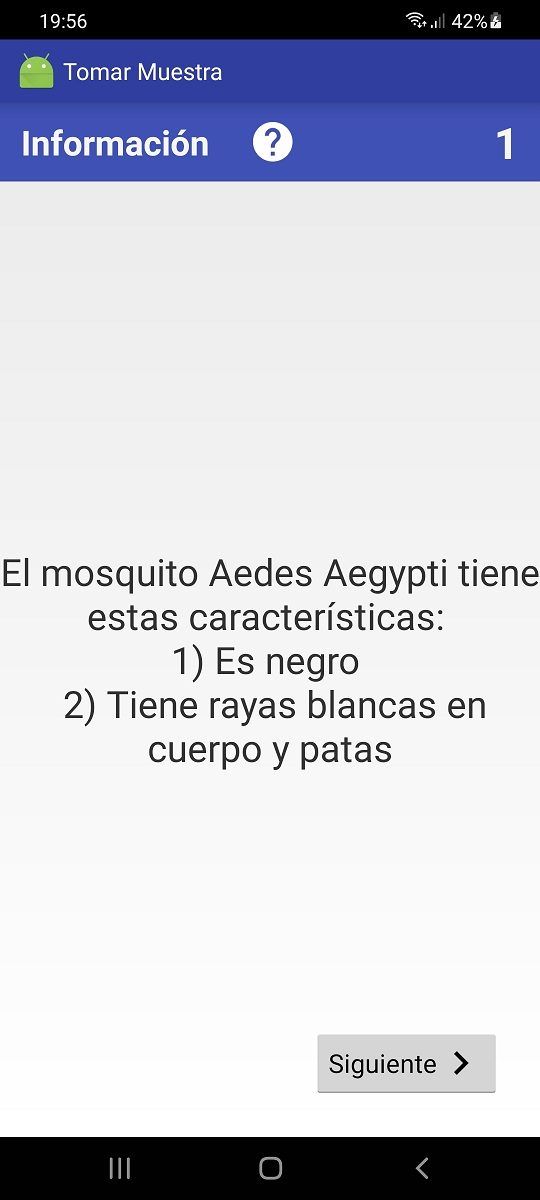
\includegraphics[scale=0.3]{05-implementacion/app_generada_ejemplo2.jpg}    
   \end{center}
   \begin{center}
   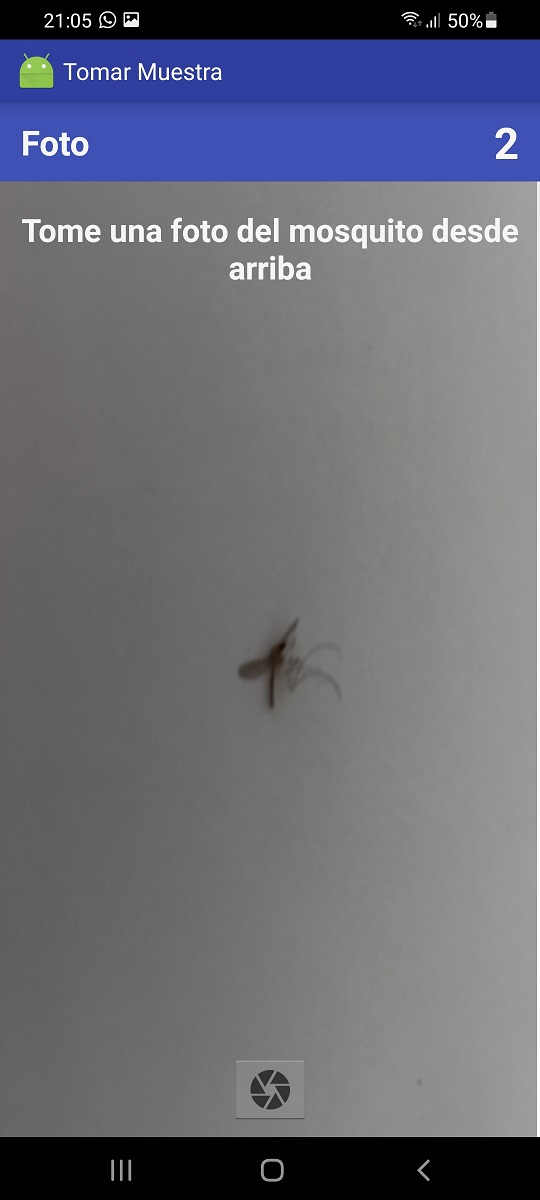
\includegraphics[scale=0.3]{05-implementacion/app_generada_ejemplo3.jpg}   
   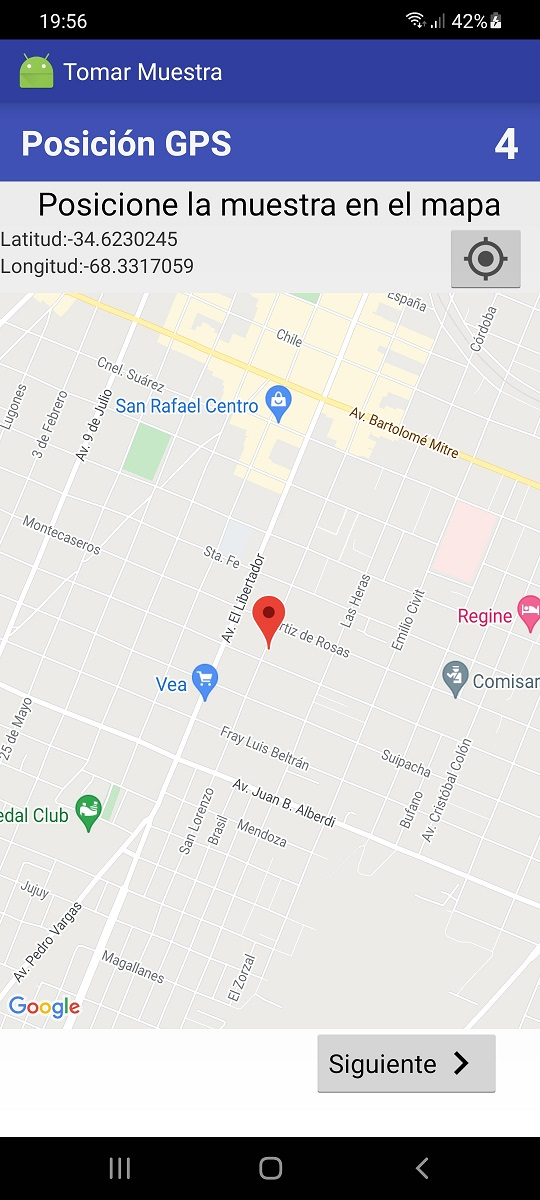
\includegraphics[scale=0.3]{05-implementacion/app_generada_ejemplo4.jpg}       
   \end{center}
   
   \caption{Capturas de pantalla de la app de ejemplo generada por Samplers}
\end{figure}




Las opciones disponibles y cómo se configura el archivo de configuración de Samplers se explican en la sección \ref{sec:archivo_configuracion}.

De esta manera un científico que desee generar una app para su proyecto de ciencia ciudadana, solo tiene que completar el archivo de configuración, ejecutar Samplers y luego compilar en Android Studio y ejecutar la app en un dispositivo móvil o en los dispositivos virtuales que provee Android Studio para debugging.

Como Samplers genera el código fuente de la app, esto permite que un usuario con conocimientos de programación pueda modificarlo y personalizar la app a su gusto, así como también agregarle otras funcionalidades a la app generada. También permite que pueda ser usado en una app ya desarrollada o en desarrollo, como si fuera una librería que se incluye al proyecto y permite usar sus clases (esto se explica con más detalle en la sección \ref{sec:usando_las_clases}).

Como Samplers se pensó como un proyecto dentro de Cientópolis\cite{cientopolis} el mismo es open source y se usó un repositorio público en GitHub\cite{github} para dejar el código fuente disponible para todo el mundo.


\begin{comment}
También provee un mecanismo de identificación del usuario final de la aplicación (el científico ciudadano) usando su cuenta de Google, ya que en los dispositivos móviles con sistema operativo Android se requiere de una cuenta de Google para acceder a muchas de las funcionalidades, como por ejemplo la Play Store (la tienda de Android para descargar aplicaciones).  Ademas esta preparado para que el usuario del framework pueda incluir su propio sistema de inicio de sesión (por ejemplo con usuario y contraseña) o con una API de alguna red social, como Facebook, Twitter, Instagram, etc.


Samplers también provee un mecanismo para mostrar ayuda asociada a un paso (Step) en particular y una ayuda general en la pantalla principal, usando archivos HTML. Se optó por los mismos por la variedad de opciones y posibilidades que conllevan, y por su simpleza para mostrarlos.
\end{comment}

\subsection{Archivo de configuración}\label{sec:archivo_configuracion}

\begin{comment}

En el objeto project, se encuentran las configuraciones del proyecto de Android Studio en el cual se creará la app, y son las siguientes:
\begin{itemize}

\item app\_path: la ruta relativa a los archivos fuente de la app. Es donde se crearán los archivos de las Activities por ejemplo.

\item package\_name: el nombre del package que se usará para las Activities de la app (generalmente ``com.example.myApplication"). 

\end{itemize}

En el objeto application, se encuentran los parámetros para configurar la app, como por ejemplo el mensaje de bienvenida o el servidor web al que se deben enviar las muestras recolectadas. Los parámetros son los siguientes:
\begin{itemize}

\item title: el título de la app.

\item welcomeMessage: el mensaje de bienvenida que se muestra en la Activity principal.  

\item networkConfiguration: la configuración del servidor al que se enviarán las muestras tomadas con la app

\begin{itemize}
\item url: la url del servidor a la cual se enviarán las muestras mediante un mensaje HTTP POST.

\item paramName: el nombre del parámetro dentro del mensaje HTTP POST que se usará para enviar la muestra.

\item paramNameUserId: [Opcional] el nombre del parámetro dentro del mensaje HTTP POST que se usará para enviar el id del usuario que tomó la muestra (si los métodos de identificación estan habilitados).

\item paramNameAuthenticationType: [Opcional] el nombre del parámetro dentro del mensaje HTTP POST que se usará para enviar el tipo de identificación que se usó (si los métodos de identificación estan habilitados).

\end{itemize}

\item googleMaps\_API\_KEY:

\item mainHelpFileName: [Opcional] se puede espe 
el nombre del archivo HTML que se usará.
The file name of the HTML file containing the main application help

\item authenticationEnabled: [Opcional] habilita los métodos de identificación del usuario que toma las muestras.

\item authenticationOptional: [Opcional] indica si la identificación (en caso de estar habilitada) será opcional u obligatoria.


\end{itemize}

\end{comment}

El archivo de configuración es un archivo en formato JSON que se debe completar con los parámetros necesarios para crear la app con Samplers. Se eligió el formato JSON porque nos pareció más sencillo de manipularlo por una persona (que XML por ejemplo, que también fue evaluado), suponiendo que el científico tuviese que editarlo manualmente.

El archivo está compuesto por tres objetos: project, application y workflow.

En el objeto project, se encuentran las configuraciones del proyecto de Android Studio en el cual se creará la app, como por ejemplo la ruta en donde se crearán los archivos de las Activities y el nombre del package que se usará para las mismas. 

En el objeto application, se encuentran los parámetros para configurar la app, como por ejemplo el título de la app, el mensaje de bienvenida o el servidor web al que se deben enviar las muestras recolectadas. 

El objeto workflow se usa justamente para configurar el Workflow (el protocolo de recolección) que usará la app para tomar las muestras. En el mismo se deben especificar los Steps que se usarán con sus respectivos parámetros cada uno. Por defecto Samplers provee los siguientes Steps:

\begin{itemize}

\item Information: Muestra un texto al científico ciudadano.

\item Photo: Solicita tomar una foto.

\item Sound: Solicita grabar sonido.

\item Location: Solicita tomar la posición del GPS del dispositivo móvil.

\item Route: Solicita grabar con el GPS del dispositivo móvil un recorrido (un conjunto de posiciones GPS).

\item SelectOne: Solicita seleccionar una única respuesta a una pregunta.

\item MultipleSelect: Solicita seleccionar una o varias respuestas a una pregunta.

\item InsertText: Solicita ingresar texto.

\item InsertDate: Solicita seleccionar una fecha.

\item InsertTime: Solicita seleccionar una hora.

\end{itemize}

En la siguiente imagen se muestra un ejemplo del archivo de configuración para Samplers.
\begin{figure}[H]
  \centering
    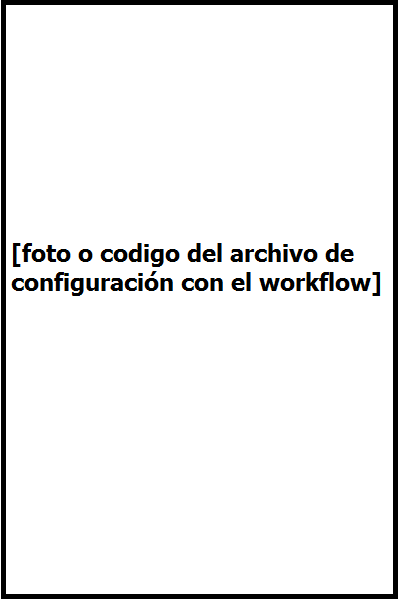
\includegraphics[width=\textwidth]{05-implementacion/archivo_config_ejemplo.png} 
   \caption{Ejemplo de un archivo de configuración para Samplers}
\end{figure}

Una vez configurado el archivo, Samplers generará una Activity principal para la app que tendrá todas las configuraciones del objeto application y que usará el Workflow configurado para llamar a la Activity encargada de tomar las muestras (TakeSampleActivity) cuando el científico ciudadano presione el botón para tomar una muestra.

El detalle de todos los parámetros, como configurar el archivo de configuración y los diferentes Steps disponibles para armar el Workflow se explican en la sección \ref{sec:archivo_config_detallado}


\subsection{Usando las clases} \label{sec:usando_las_clases}
Como se mencionó antes, Samplers también puede ser usado por una persona con conocimientos de programación en una app que se encuentre en desarrollo, como si fuera una librería que se incluye al proyecto y permite usar sus clases. 

Básicamente se tiene que instanciar la clase Workflow y agregarle instancias de los diferentes Steps que se quieran usar. Luego, en el método «onClick» de algún botón, iniciar la Activity TakeSampleActivity pasándole como parámetro la instancia de Workflow creada. De esta forma, cuando se presione dicho botón, Samplers se encargará te tomar la muestra, guardarla en el dispositivo móvil y enviarla al servidor cuando haya conexión wifi.

\begin{figure}[H]
  \centering
    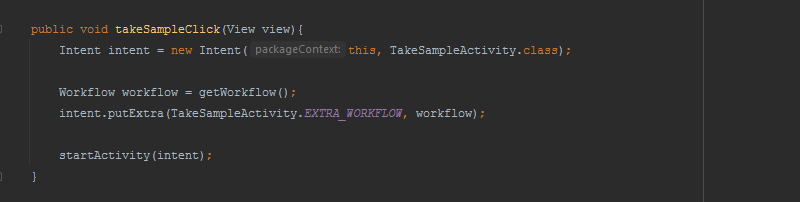
\includegraphics[scale=0.6]{05-implementacion/take_sample_click.png} 
   \caption{Ejemplo de como iniciar la activity TakeSampleActivity instanciando las clases.}
\end{figure}	

El detalle de como usar las clases y establecer las configuraciones adicionales se explican en la sección \ref{sec:instanciacion_manual}.

\section{Estructura e implementación del Framework}

Samplers está compuesto por dos elementos: una librería con las clases y demás recursos necesarios para crear la app y un script en Gradle para procesar el archivo de configuración.

La librería es un archivo .aar, que es similar a un archivo .jar de Java, pero especifico para Android. En el mismo están todas las clases y los archivos de recursos de Android (como archivos XML con los diseños de IU de los Fragments y Activities, iconos, imágenes, etc).

El script de Gradle es el que procesa el archivo de configuración de Samplers (SamplersConfig.json) y genera la app correspondiente usando las clases y recursos de la librería.

A continuación se explican las clases y componentes de Android que permiten que se cree una aplicación móvil con Samplers y su funcionamiento, y como se resolvieron cuestiones como el almacenamiento y envió de las muestras, la identificación de los usuarios que envían las muestras, etc.

\subsection{Workflow, Step, StepFragment, StepResult, Sample} \label{sec:clases_core}
Estas clases conforman el corazón del framework, y son las necesarias para poder definir el protocolo de recolección de las muestras.

A continuación se muestra el diagrama de clases (Figura \ref{fig:umlFrameworkCore}).

\begin{figure}[H]
  \centering
    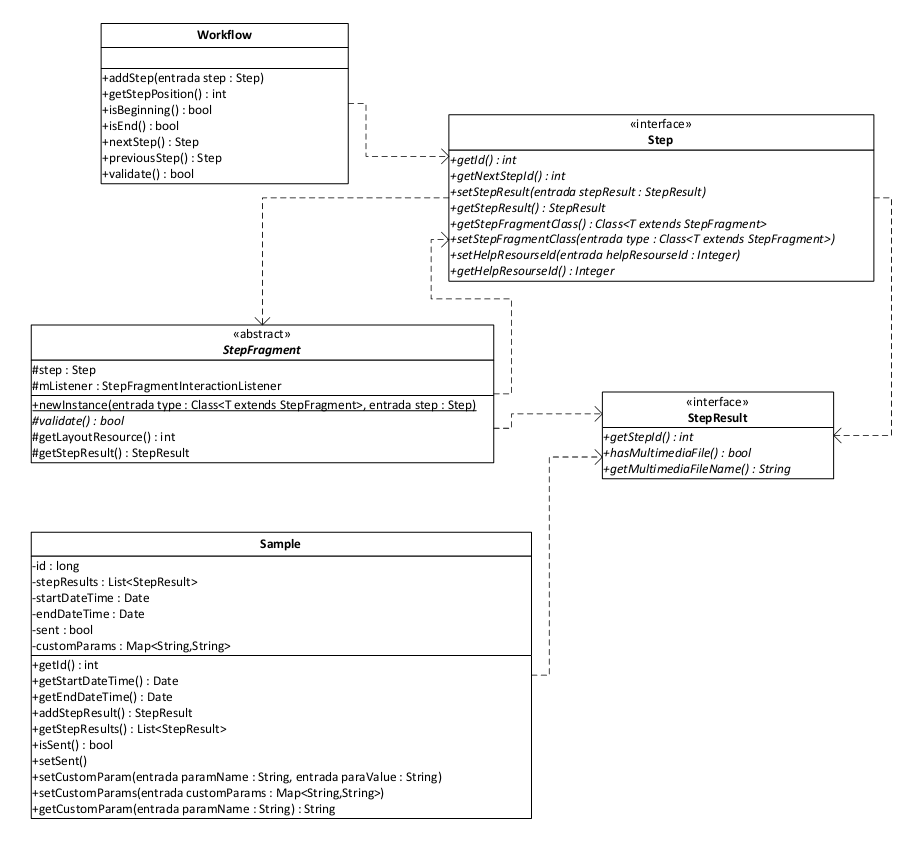
\includegraphics[scale=0.4]{05-implementacion/FrameworkCore.png} 
   \caption{Diagrama de clases del core del framework}
   \label{fig:umlFrameworkCore}
\end{figure}


TakeSampleActivity es una Activity y es la encargada de tomar la muestra.
Recibe como parámetro un Workflow, que representa el protocolo de recolección de la muestra.
El Workflow esta formado por varias instancias de Step, que representan cada una un paso a seguir dentro del protocolo de recolección para obtener la muestra.

TakeSampleActivity ejecuta el Workflow y por cada Step obtiene y muestra en pantalla el StepFragment asociado, que es el Fragment encargado de mostrar la interfaz de usuario para ejecutar ese Step. 
El StepFragment a través de la interacción con el usuario final (el científico ciudadano) genera un StepResult, que es el resultado de la ejecución del Step asociado. Por cada tipo de Step, debe haber una clase StepFragment que sepa ejecutar ese Step y generar el StepResult asociado.

El conjunto de todos los StepResults obtenidos después de ejecutar todos los Steps del Workflow forman la muestra, que esta representada por la clase Sample.


\subsubsection{Workflow: el protocolo de recolección de las muestras}
La clase Workflow representa el protocolo de recolección de las muestras. Está formado por una colección de Steps, que representan los pasos a seguir para completar dicho protocolo, y un Step inicial que indica el inicio del mismo (el primer Step a ejecutar).

El Workflow es el encargado de llevar el estado del paso en el que se encuentra, y posee métodos para obtener el siguiente Step (\textit{nextStep()}  que depende del Step actual) y el Step anterior (\textit{previuosStep()}  para lo que maneja una lista a modo de pila\footnote{Pila o stack en inglés, una lista ordenada con acceso a sus elementos de tipo «último en entrar, primero en salir»}).

El Workflow se comporta de manera secuencial, puede ir hacia adelante o volver hacia atrás, pero esto no impide que pueda tener bifurcaciones, y así formar diferentes caminos para tomar la muestra. Por ejemplo, se le podría preguntar al científico ciudadano si observa una característica particular al momento de tomar la muestra, y si la observa solicitarle que tome una foto de la misma, pero en caso contrario se puede omitir el paso de la foto.

\subsubsection{Step: el paso}
Un Step representa un paso dentro del Workflow. Tiene asociado un StepFragment que es el encargado de ejecutar el Step para generar un StepResult (el resultado). El Step básicamente tiene los parámetros o información para que pueda ser ejecutado por el StepFragment.
Por ejemplo, para el caso en que el paso sea contestar una pregunta, el Step tendrá la pregunta en sí (un String) y una colección con las posibles respuestas (id y descripción).

El Step conoce cuál es el siguiente Step a ejecutar aunque a veces éste depende del StepResult generado, como es el caso de SelectOneStep en el que el siguiente paso depende de la opción seleccionada, y con esto se pueden crear bifurcaciones en el Workflow.

Samplers provee los siguientes Steps:
\begin{itemize}
	\item InformationStep: Muestra una información (texto) al usuario.
	\item PhotoStep: Permite tomar una foto con la cámara del dispositivo móvil.
	\item SoundRecordStep: Permite grabar un sonido con el micrófono del dispositivo móvil.
	\item SelectOneStep: Muestra una pregunta con varias opciones como respuesta, de las cuales solo se puede seleccionar una sola.
	\item MultipleSelectStep: Muestra una pregunta con varias opciones como respuesta, de las cuales solo se pueden seleccionar varias opciones.
	\item LocationStep: Permite tomar la geo posición del dispositivo móvil.
	\item RouteStep: Permite grabar un recorrido usando el GPS del dispositivo móvil.
	\item InsertTextStep: Permite ingresar un texto.
	\item InsertDateStep: Permite seleccionar una fecha.
	\item InsertTimeStep: Permite seleccionar una hora.
\end{itemize}

El detalle de estos Steps y su funcionamiento se explican en la sección \ref{sec:steps_detallados}.

Si bien estos son los Steps que provee Samplers de manera predeterminada, un usuario programador puede definir y agregar sus propios Steps, junto con sus StepFragments y StepResults como se explica en la sección \ref{sec:definir_steps}.

\subsubsection{StepFragment: la vista y controlador del Step}
El StepFragment es el encargado de ejecutar un Step y generar un StepResult con la interacción del usuario final (el científico ciudadano). Un StepFragment recibe un Step, que generalmente contiene los parámetros necesarios para ejecutarlo, y en base a eso muestra un Fragment para que, interactuando con el científico ciudadano, poder obtener un resultado (StepResult) para la muestra (Sample). 

Por ejemplo, para el caso en que el paso sea contestar una pregunta, se mostrará la pregunta y se listarán las posibles respuestas en forma de radio-buttons, si solo se admite seleccionar una única respuesta, o en forma de check-buttons, si se permite seleccionar más de una.

Por cada tipo de Step, debe haber una clase StepFragment que sepa ejecutar ese Step y generar el StepResult asociado.

Es una clase abstracta, ya que su comportamiento depende de la implementación de cada tipo de StepFragment que se defina. Se definió así y no como una interfaz por la necesidad de que heredara de Fragment porque así lo necesita la Activity TakeSampleActivity, que es la encargada de ejecutar el Workflow para tomar la muestra.

Por cada Step que provee Samplers de manera predeterminada, también se provee un StepFragment que ejecuta cada Step. Asimismo, un usuario programador también puede desarrollar un StepFragment propio para alguno de los Steps provistos por Samplers, como se explica en la sección \ref{sec:definir_steps}



\subsubsection{StepResult: el resultado de la ejecución de un Step}
El StepResult representa el resultado que se obtiene de ejecutar un Step. Contiene los datos obtenidos de ejecutar el Step asociado. Cada ejecución de un mismo Step, puede generar un StepResult diferente.

Por ejemplo, para el caso en que el Step sea contestar una pregunta, el StepResult contendrá la respuesta seleccionada, si solo se admite seleccionar una única respuesta, o una colección de respuestas, si se permite seleccionar más de una.

Se definió como una interfaz, ya que su comportamiento depende de la implementación de cada tipo de Step que se defina.

Un StepResult tiene asociado el Step en base al cual se generó. También puede tener asociado un archivo multimedia, como por ejemplo en los casos de PhotoStep y SoundRecordStep que guardan una foto y un archivo de sonido respectivamente.


\subsubsection{Sample: la Muestra}
La clase Sample representa una muestra tomada a partir de seguir los pasos (Steps) del protocolo del recolección (Workflow). Contiene los resultados (StepResult) de la ejecución de cada paso. Cada ejecución del Workflow puede generar una colección de StepResults diferente.

También guarda fecha y hora de inicio y finalización. Esto es útil para sacar una estadística de cuanto tarda un científico ciudadano en recolectar una muestra y así poder analizar optimizaciones para la aplicación final.

Una vez recolectadas, las muestras se guardan en el dispositivo móvil y son enviadas a través de Internet a un servidor web previamente configurado.

\subsection{TakeSampleActivity}
La clase TakeSampleActivity es la encargada de ejecutar el Worflow para tomar la muestra. Es una Activity que recibe un objeto Workflow como parámetro y va iterando sobre los Steps del mismo. A cada Step le pide su StepFragment y lo muestra en pantalla para que, interactuando con el científico ciudadano, se genere el StepResult para la muestra (Sample). Una vez finalizado el Workflow, guarda la muestra, controla si se puede enviar la misma y finaliza.



\subsection{Persistencia local}\label{sec:persistencia_local}
Las muestras se guardan en el dispositivo móvil en un archivo JSON, junto con los archivos multimedia que pudiera tener, dentro de un directorio por cada muestra. Las mismas se guardan dentro del directorio «samples» en el almacenamiento interno del dispositivo.

Se eligió el almacenamiento interno para guardar las muestras porque no se necesitan permisos especiales para acceder al mismo y, de forma predeterminada, los archivos que se guardan en el mismo son privados para la aplicación y otras aplicaciones no pueden tener acceso a ellos (tampoco el usuario). Cuando el usuario desinstala la aplicación, estos archivos se quitan\cite{androidInternalStorage}.

Por ejemplo, una muestra con id 123456 y 2 fotos se guarda de la siguiente manera:

\begin{figure}[H]
  \centering
    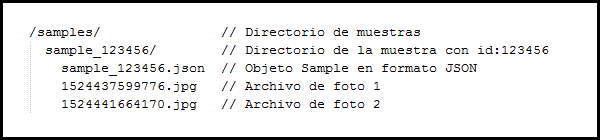
\includegraphics[scale=0.8]{05-implementacion/persistencia_local.png} 
   \caption{Ejemplo de cómo se guarda una muestra.}
\end{figure}		

Para pasar la muestra a un archivo JSON se usó Gson\cite{gson}, una librería de Google distribuida bajo licencia Apache 2.0 que convierte objetos Java a JSON y viceversa de manera muy sencilla, con métodos \textit{toJson()} y \textit{fromJson()} para convertir hacia y desde JSON respectivamente.

\subsection{Envío de muestras a servidor web}\label{sec:envio_muestras}

Una vez guardadas localmente, las muestras se envían al servidor web previamente configurado, mediante un mensaje HTTP POST. Para ello se usó la librería OkHttp\cite{okhttp}, distribuida por Square Inc. bajo licencia Apache 2.0, que resuelve de manera sencilla y eficiente el envío de mensajes HTTP en Android.

Por cada muestra se envía el objeto Sample en formato JSON junto con los archivos multimedia que pudiera tener, todo comprimido en un solo archivo ZIP. Para comprimir las mismas se usaron las librerías estándares de Java (java.util.zip) que proporciona clases para leer y escribir archivos ZIP y GZIP estándares.

Las muestras se envían automáticamente cuando se detecta conexión wifi o a petición del usuario usando cualquier red disponible.

En el caso de envío automático, luego de guardar la muestra se controla si el dispositivo está conectado a una red wifi y se intenta enviar la muestra; caso contrario queda pendiente de envío y se intenta enviar cuando se detecta conexión wifi. Para detectar la conexión a wifi se usa un BroadcastReceiver que atiende el evento de difusión que envía Android cuando el dispositivo móvil se conecta a wifi, aún cuando la app no se esté ejecutando, lo que permite el envío de la muestra con un Service en segundo plano.

Para el caso que es a petición del usuario, se listan las muestras tomadas en la Activity SamplesListActivity con un botón que permite el envío de las mismas usando cualquier tipo de conexión a Internet.

\subsection{Identificación}
Samplers provee un sistema de identificación (login), el cual se puede habilitar o no de acuerdo a las necesidades del proyecto. Si se habilita el mismo puede ser opcional, permitiendo al científico ciudadano tomar y enviar muestras habiéndose o no identificado, o puede ser obligatorio, requiriendo que el científico ciudadano se identifique para poder tomar y enviar las muestras.

De manera predeterminada Samplers incluye identificación con la API de Google, es decir que el científico ciudadano puede usar su cuenta de Google que tiene configurada en el dispositivo móvil Android para identificarse en la aplicación.

Además, un usuario programador del framework puede definir su propio método de identificación, ya sea con usuario y contraseña o usando alguna otra API de redes sociales por ejemplo, como son Facebook, Instagram, Twitter, etc. como se explica en la sección \ref{sec:usar_auth_propia}.

Cuando se envía la muestra también se incluyen dos parámetros que son el id del usuario identificado y el método usado para identificar (que puede ser google o uno personalizado). Se envían de esta forma porque al momento de tomar la muestra el científico ciudadano puede no estar identificado, e identificarse antes de enviarlas.

\subsection{Otras Activities de la app generada por Samplers}
Como se mencionó antes, Samplers genera una app lista para ejecutar en un dispositivo móvil con Android, por lo que se incluyen otras Activities para completar la app generada. A continuación se describen dichas Activities

\subsubsection{SamplersMainActivity}
SamplersMainActivity es la Activity principal de la app generada, es la que se inicia cuando el usuario hace clic sobre el icono de la app. Esta Activity contiene la pantalla principal de la app, en la que se muestra el mensaje de bienvenida configurado, un menú para acceder a las Activities que se explican mas abajo, y un botón para tomar la muestra que cuando se presiona se llama a TakeSampleActivity para tomar la muestra. También, si se configuró el uso de identificación, se muestra un botón para que el usuario final pueda iniciar sesión.

\begin{figure}[H]
  \centering
    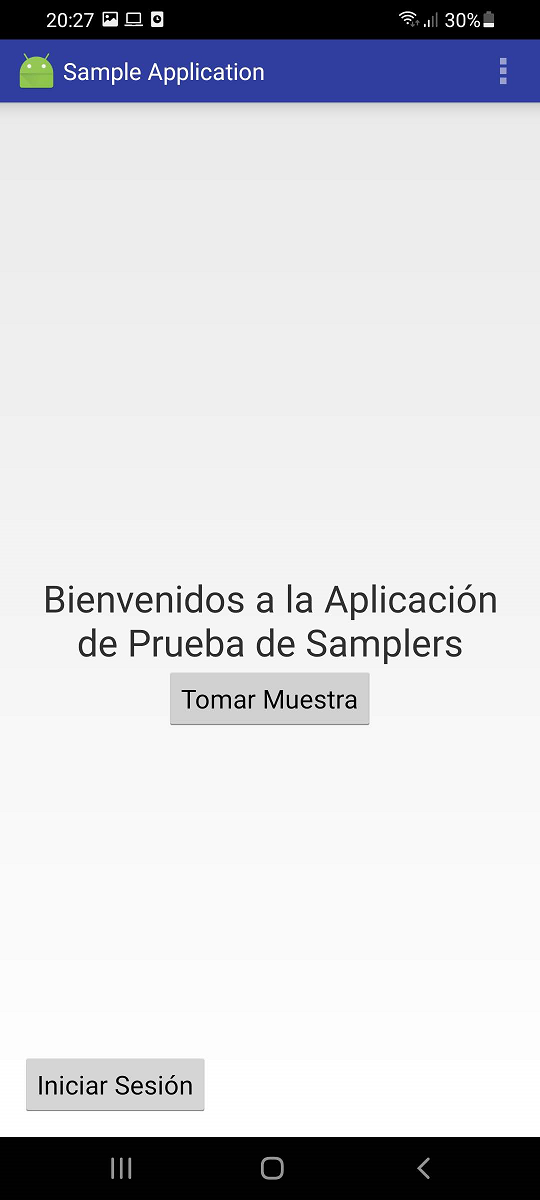
\includegraphics[scale=0.3]{05-implementacion/SamplersMainActivity.png} 
   \caption{Ejemplo de la Activity principal.}
\end{figure}	



\subsubsection{SamplesListActivity}
SamplesListActivity es una Activity que visualiza un listado de las muestras tomadas por el usuario final de la app, y que se encuentran almacenadas en el dispositivo móvil, con opciones para eliminarlas o enviarlas al servidor en caso de que no hayan sido enviadas automáticamente.

\begin{figure}[H]
  \centering
    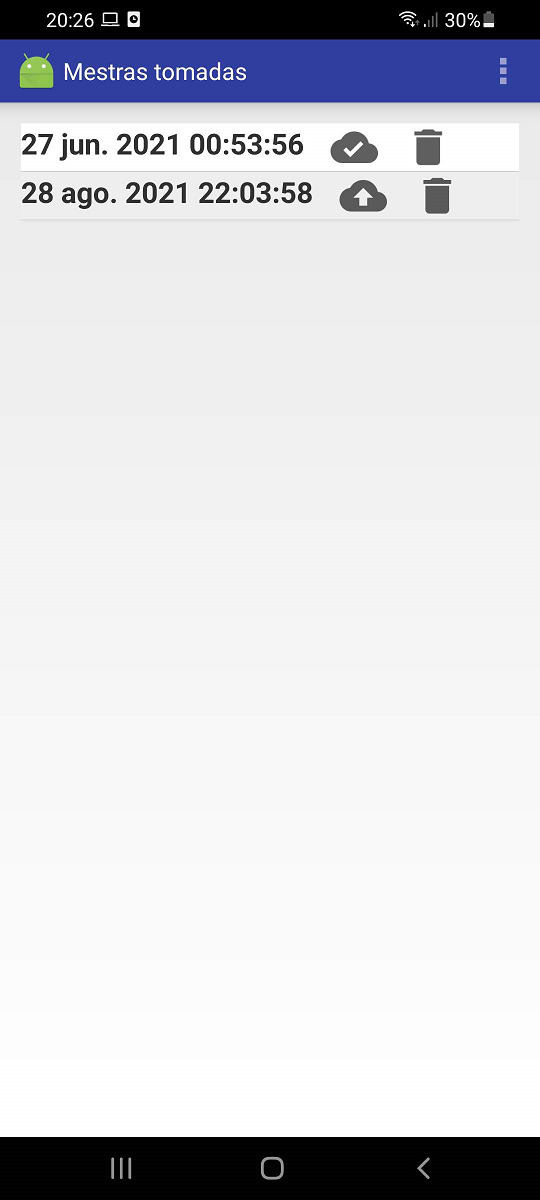
\includegraphics[scale=0.3]{05-implementacion/SamplesListActivity.png} 
   \caption{Ejemplo de como se visualiza SamplesListActivity.}
\end{figure}	


\subsubsection{HelpActivity}
HelpActivity es una Activity que se usa para mostrar ayuda al usuario final de la app. Para mostrar ayuda se debe configurar la misma en formato HTML como se explica en la sección \ref{sec:mostrar_ayuda}. HelpActivity es la Activity que muestra tanto la ayuda general (que se accede desde el menú de SamplersMainActivity) como la ayuda que se muestra en cada StepFragment (si se configura) al momento de tomar la muestra.

\begin{figure}[H]
  \centering
    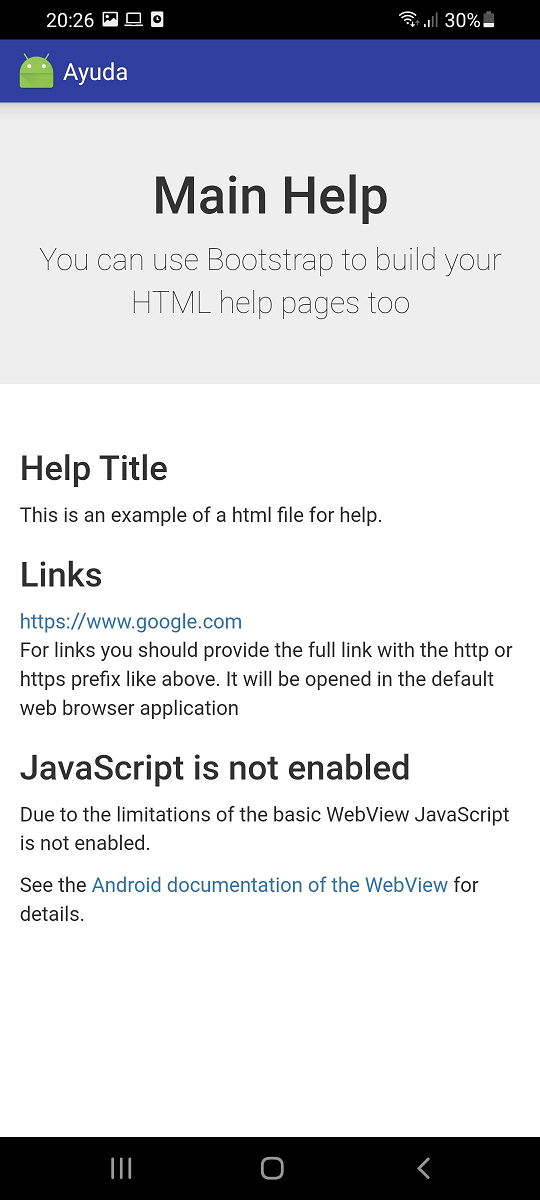
\includegraphics[scale=0.3]{05-implementacion/HelpActivity.png} 
   \caption{Ejemplo de como se visualiza SamplesListActivity.}
\end{figure}	







